\subsection{Setup}
Dasgupta et al. \cite{dasgupta2012social} performed various experiments to compare the performance of the presented samplers.
They focused on two large, publicly available databases \texttt{LiveJournal} and \texttt{DBLP}.
Note that the graphs in the following chapter are directly copied from their published paper.

The \texttt{LiveJournal} network contains 5.36M nodes and approximately 160M edges and is based on a snapshot of the social network \url{http://livejournal.com} in March 2008. In addition to the network they extracted the users' age, location (city, state, country) and a list of interests where available on the users' public profiles. They used additional filter techniques to remove invalid entries, lowering the amount of nodes to 40\%-60\% per attribute.

The \texttt{DBLP} network contains 368K nodes and 8M edges and consists of the content of the DBLP database located at \url{http://www.informatik.uni-trier.de/~ley/db/}. The nodes stand for authors while the edges represent co-authorship on some publication. The node attributes are formed by the authors publication venues, however only a random set of 100 venues with probability proportional to their popularity were considered. 

Since the samplers have been designed keeping the Definition \ref{defsampler} in mind, recall that they provide an additive $\epsilon$-approximation. So most importantly Dasgupta et al. measure the absolute error of each sampler with respect to the true value. If an estimator outputs $\hat{f}$ approximating $\bar{f}$ they measure the error as $|\bar{f}-\hat{f}|$.

To get a relation between error and sample size they vary the sample size $r$ from a minimum of $r = 100$ to $r = 50000$. They use the distributions mentioned in chapter \ref{algorithms}: uniform at random (\texttt{unif}), proportional to the degree of the node (\texttt{deg}) and additionally, proportional to the square root of the degree of the node (\texttt{sqrtdeg}). Note that in case of the \texttt{Sparse} sampler $k = 5$ has been used.
They omit any other combinations of algorithm and distributions since they almost always did not result in better performance and are computationally more expensive. 
The results were achieved using a median of means approach. This is commonly used when doing these kinds of measurements and works in the following way: one creates $l$ partitions called $A_1,...,A_l$ of the set of samples $A$. $l$ is a parameter and in this case $l = $1,3,5,7 and 9 have been used. Next, for each $l$ the median is calculated from applying the estimator to $A_1$ until $A_l$. The final result and the one presented in the graphs is the mean of these medians from all $l$.
This considers choosing partitions at random and prevents the need to specify the partition strategy when comparing the different samplers.

\subsection{Performance on LiveJournal}
For analyzing the performance on LiveJournal they are interested in a set of five cities, five states, five countries, a set of ages (20, 25, 30, 35 and 40), age-buckets ([20,29),...,) and a set of interests (various sports) each with a typical size ranging from 0.4\% to 4\%.
The correlation between number of samples and absolute error for the presented samplers is displayed in \rfig{livejournal1}.

As expected, in all scenarios, the error decreases faster than linearly with an increased number of samples.
Generally \texttt{deg} and \texttt{sqrtdeg} show similar performance and I will not discuss the details in this paper.
To get a feeling on $r$ in relation to the whole network, keep in mind that when sampling 10000 nodes one is already sampling 2\% (on average) of the whole network's nodes, an already significant sample size.

In all attributes the \texttt{Ideal} sampler shows the best performance, for example in cities until about 10000 samples its error is about half as \texttt{Naive}'s.
\texttt{Naive} generally performs better than \texttt{Expec} but surprisingly at states and countries it performs similar to the \texttt{Ideal} estimator.
The \texttt{Sparse} sampler is usually similar to the \texttt{Naive} approach with being better at cities and worse at the states attribute.
Most interestingly \texttt{Expec} shows a very indifferent performance. Out of all algorithms it seems to have the highest non-monotone behavior at around $r=200$. It is assumed that this is due to \texttt{Expec} having the highest variance because of the discretization of the value returned by each sampled node.
%---figure network a------------------------------------
\begin{figure}[!ht]
  \begin{center}
    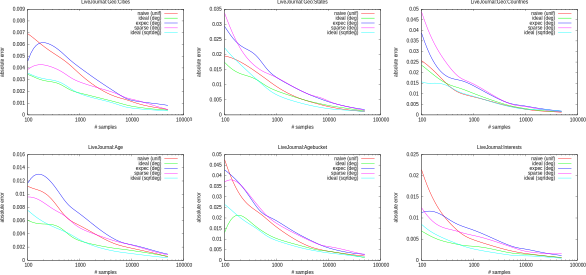
\includegraphics[width=\linewidth]{fig2_3}
    \caption{\#samples vs error of various samplers on the LiveJournal data \cite{dasgupta2012social}}
    \lfig{livejournal1} 
  \end{center}
\end{figure}
%---end figure network a--------------------------------
\subsection{Performance on DBLP}
In DBLP they are interested in 100 venues of publication ranging in size from 0.01\% to 3\% in size. The correlation between sample size and absolute error is drawn in \rfig{dblp}.

The improvements offered by \texttt{Ideal} over \texttt{Naive} are even larger. In comparison the \texttt{Naive} sampler requires at least 3-5 times more samples than \textit{Ideal} for achieving the same error.
%---figure network a------------------------------------
\begin{figure}[!ht]
  \begin{center}
    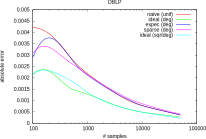
\includegraphics[width=0.5\linewidth]{fig4}
    \caption{\#samples vs error of various samplers on the DBLP data \cite{dasgupta2012social}}
    \lfig{dblp}
  \end{center}
\end{figure}
%---end figure network a--------------------------------
\subsection{Effect of sparsity parameter}
When designing the \texttt{Sparse} sampler Alg. \ref{algsparse} I introduced a new parameter $k$ which I call the sparsity parameter since it defines the amount of the picked neighbors.
The measurements displayed in \rfig{sparsity} show that using $k=9$ does not lower the error significantly, especially considering sample sizes above 400.
The authors of these experience and me assume this is related to the fact that the network has strong connectivity properties.
%---figure network a------------------------------------
\begin{figure}[!ht]
  \begin{center}
    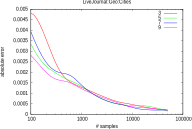
\includegraphics[width=0.5\linewidth]{fig7b}
    \caption{\#samples vs error with different sparsity parameters \cite{dasgupta2012social}}
    \lfig{sparsity}
  \end{center}
\end{figure}
%---end figure network a--------------------------------
